\label{ExercisesforIntroLimits}

\begin{enumerate}

\item  Consider the complete graph of the function $f$ below.  Use the graph to find the indicated values.

\smallskip

If a limit fails to exist, state that is the case  or use the symbols `$\infty$' or `$-\infty$' appropriately.
 
 \smallskip
 
 \textbf{NOTE:}  The graph has a vertical asymptote $x=3$.  

\begin{center}

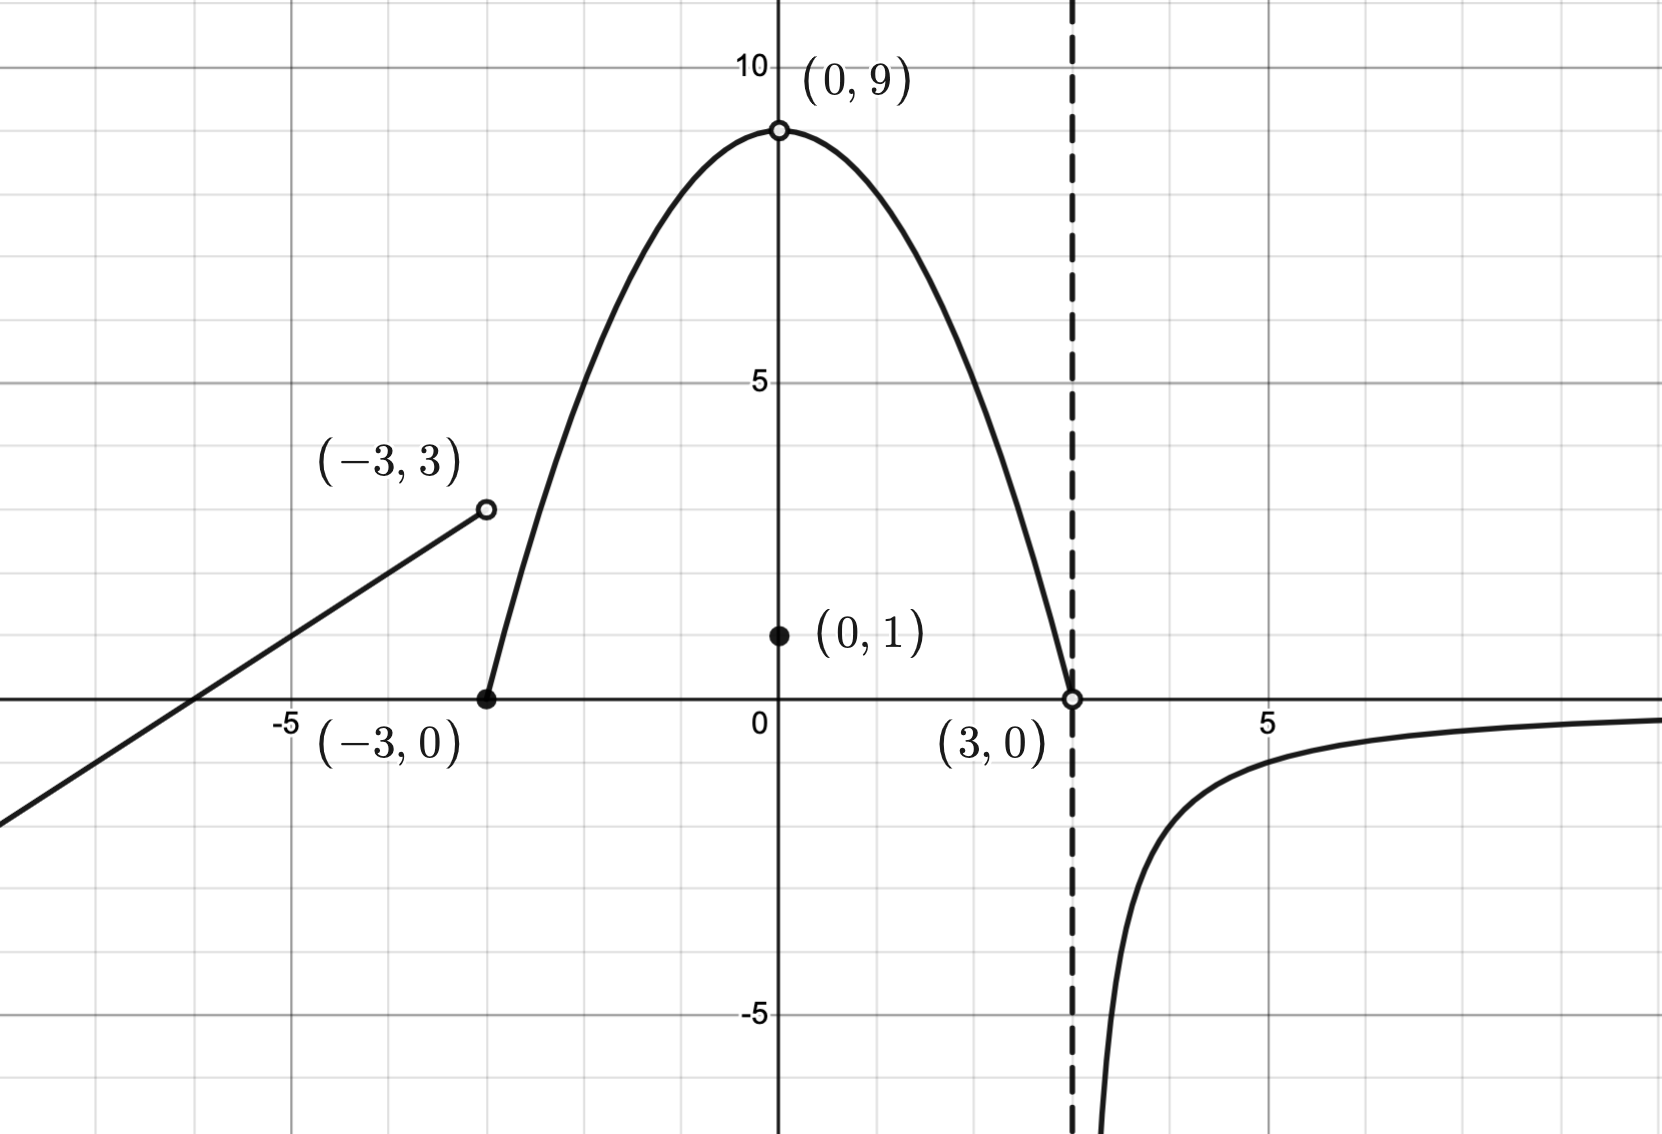
\includegraphics[width=5.5in]{./IntroLimitsGraphics/M2500TH01.png}

\end{center}

\bigskip

\begin{multicols}{4}

\begin{itemize}

\item $\ds{\lim_{x \rightarrow -3^{-}} f(x)}$

\item $\ds{\lim_{x \rightarrow -3^{+}} f(x)}$

\item $\ds{\lim_{x \rightarrow -3} f(x)}$

\item $f(-3)$

\end{itemize}

\end{multicols}

\bigskip

\begin{multicols}{4}

\begin{itemize}

\item $\ds{\lim_{x \rightarrow 0} f(x)}$

\item  $f(0)$

\item $\ds{\lim_{x \rightarrow 3^{-}} f(x)}$

\item $\ds{\lim_{x \rightarrow 3^{+}} f(x)}$
\end{itemize}

\end{multicols}

\bigskip


\item\label{twosidedonesidedlimitexistexercise}  \begin{enumerate}  \item  Explain why if $\ds{\lim_{x \rightarrow a} f(x)}$ exist, then so do $\ds{\lim_{x \rightarrow a^{-}} f(x)}$ and $\ds{\lim_{x \rightarrow a^{+}} f(x)}$.

\item   Find an instance\footnote{There are a few examples to be found in Example \ref{limitfromgraphex} \ldots}  where   $\ds{\lim_{x \rightarrow a^{-}} f(x)}$ and $\ds{\lim_{x \rightarrow a^{+}} f(x)}$ both exist but $\ds{\lim_{x \rightarrow a} f(x)}$ does not.

\end{enumerate}

\item  Consider the complete graph of the function $g$ below.  Use the graph to find the indicated values.

\smallskip


If a limit fails to exist, state that is the case  or use the symbols `$\infty$' or `$-\infty$' appropriately.
  
\smallskip

 
 \textbf{NOTE:}  The graph has a vertical asymptote $x=-2$ and a horizontal asymptote $y = 1$.  



\begin{center}

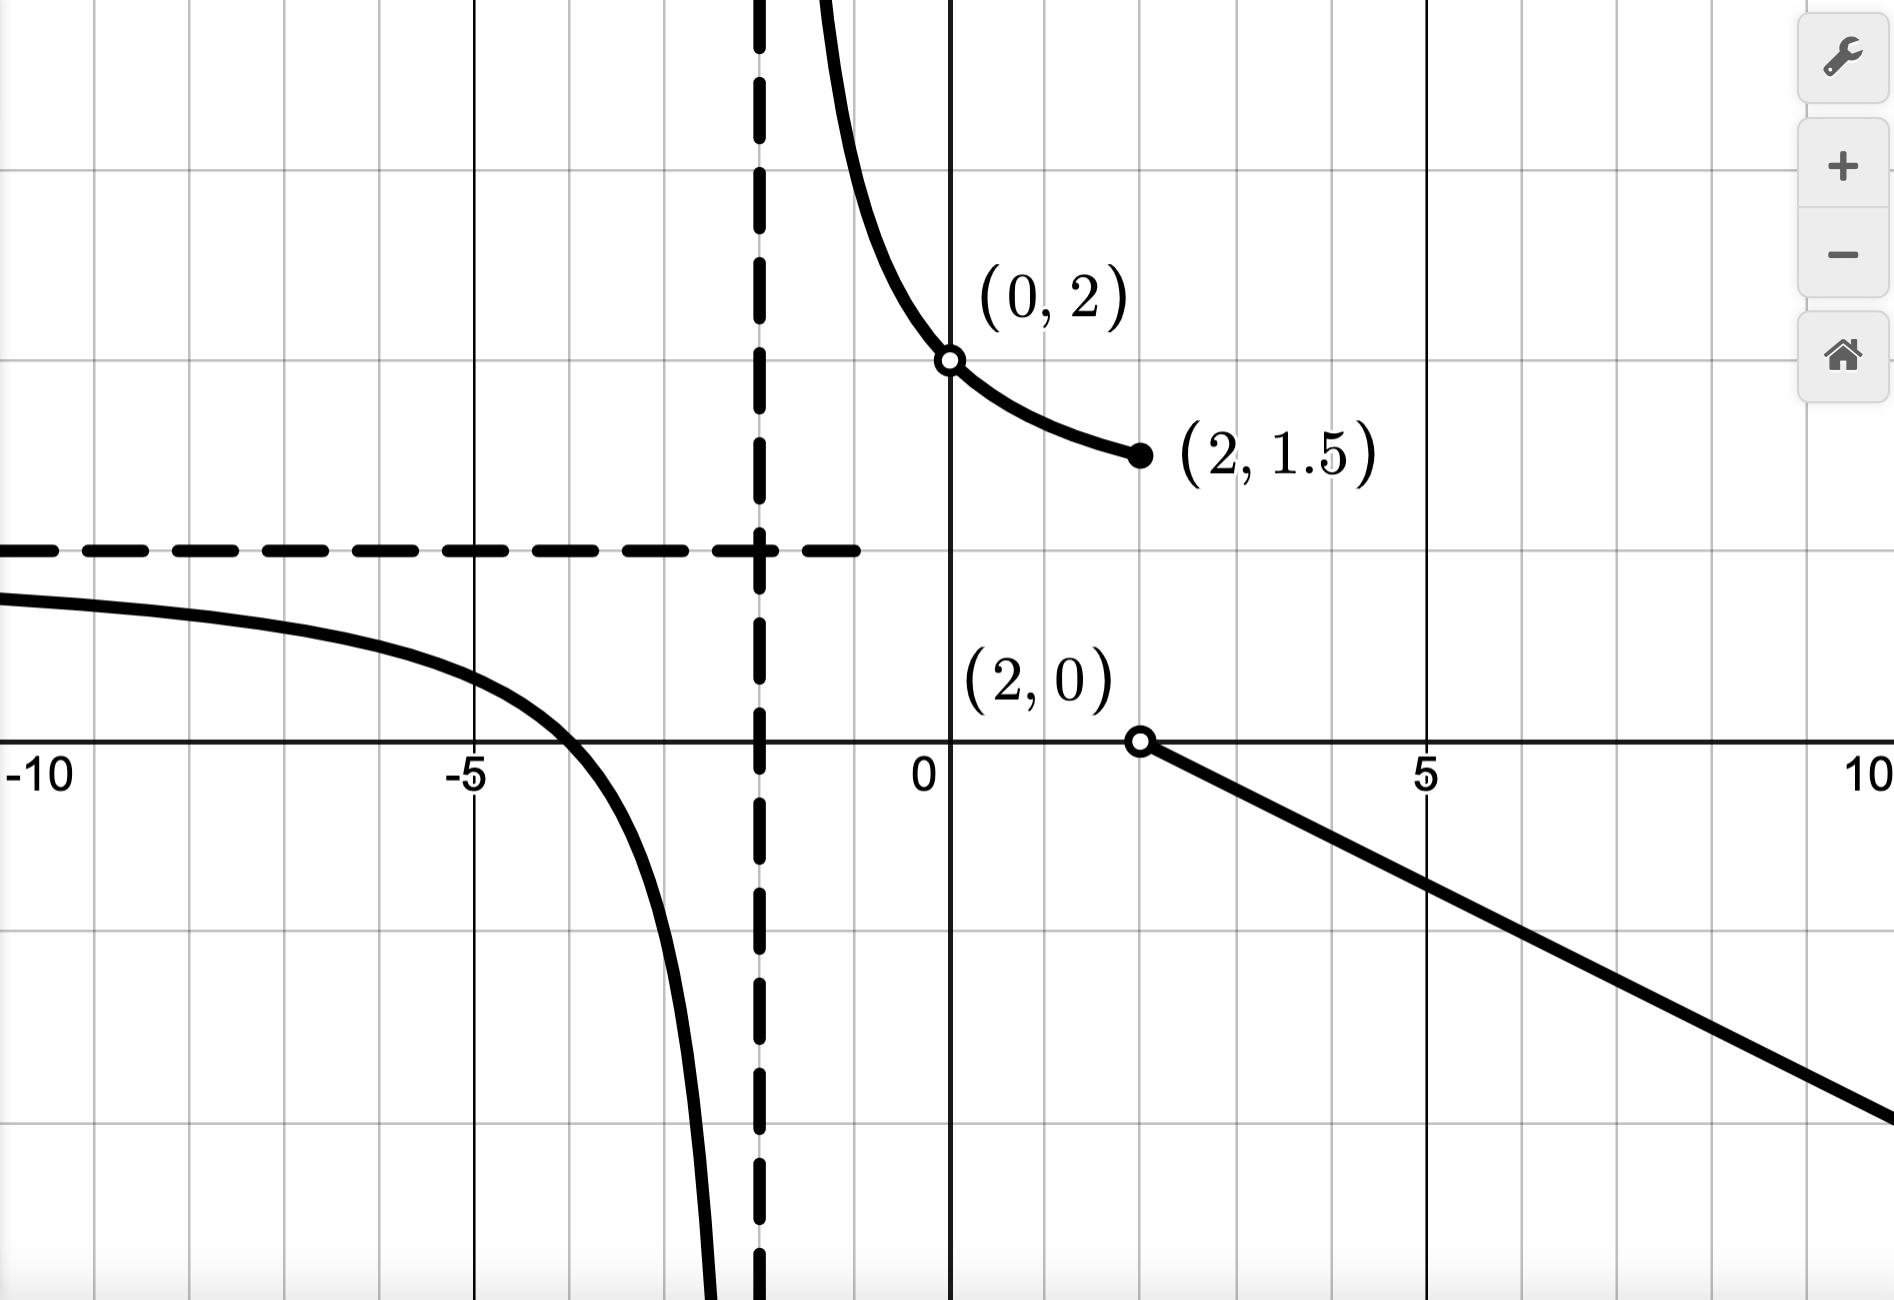
\includegraphics[width=5.5in]{./IntroLimitsGraphics/M2500_T01_Sp25_a.png}

\end{center}

\bigskip

\begin{multicols}{4}

\begin{itemize}

\item $\ds{\lim_{x \rightarrow -\infty} g(x)}$

\item $\ds{\lim_{x \rightarrow -2^{-}} g(x)}$

\item $\ds{\lim_{x \rightarrow -2^{+}} g(x)}$

\item  $\ds{\lim_{x \rightarrow \infty} g(x)}$

\end{itemize}

\end{multicols}

\bigskip

\begin{multicols}{4}

\begin{itemize}

\item $\ds{\lim_{x \rightarrow 0} g(x)}$

\item $\ds{\lim_{x \rightarrow 2^{-}} g(x)}$

\item  $g(2)$

\item $\ds{\lim_{x \rightarrow 2^{+}} g(x)}$
\end{itemize}

\end{multicols}

\bigskip

\setcounter{HW}{\value{enumi}}
\end{enumerate}

For Exercises \ref{factorcancelfirst} - \ref{factorcancellast}, find the limit analytically using Exercise \ref{rationallimit} as a guide.  If a limit fails to exist, state that is the case  or use the symbols `$\infty$' or `$-\infty$' appropriately.
 
\begin{multicols}{3}

\begin{enumerate}
\setcounter{enumi}{\value{HW}}

\item\label{factorcancelfirst}  $\ds{\lim_{x \rightarrow 2} \dfrac{2x^2+x-3}{x^2-1}}$
  
\item  $\ds{\lim_{x \rightarrow 1} \dfrac{2x^2+x-3}{x^2-1}}$

\item   $\ds{\lim_{x \rightarrow -1} \dfrac{2x^2+x-3}{x^2-1}}$

\setcounter{HW}{\value{enumi}}
\end{enumerate}

\end{multicols}

\begin{multicols}{3}

\begin{enumerate}
\setcounter{enumi}{\value{HW}}

\item   $\ds{\lim_{x \rightarrow -1^{+}} \dfrac{2x^2+x-3}{x^2-1}}$

\item  $\ds{\lim_{x \rightarrow 3} \dfrac{x^2-3x}{x^2-x-6}}$

\item\label{factorcancellast}  $\ds{\lim_{x \rightarrow 3} \dfrac{x^2-6x}{x^2-6x+9}}$

\setcounter{HW}{\value{enumi}}
\end{enumerate}

\end{multicols}

For Exercises \ref{abscancelfirst} - \ref{abscancellast}, use the piecewise definition of absolute value, Definition \ref{absolutevaluepiecewise} to help you find the limit analytically.    If a limit fails to exist, state that is the case  or use the symbols `$\infty$' or `$-\infty$' appropriately.

\begin{multicols}{2}
\begin{enumerate}
\setcounter{enumi}{\value{HW}}

\item\label{abscancelfirst} $\ds{ \lim_{x \rightarrow 3^{-}} \dfrac{|3x - x^2| }{x-3}}$     

\item\label{abscancellast}  $\ds{\lim_{x \rightarrow 2^{+}} \dfrac{|6-3x|}{x^2-4x+4}}$

\setcounter{HW}{\value{enumi}}
\end{enumerate}
\end{multicols}

For Exercises \ref{complexcancelfirst} - \ref{complexcancellast}, simplify the complex fraction in order to help you find the limit analytically.\footnote{A review of Section \ref{AppRatExpEqus} may be in order.}  If a limit fails to exist, state that is the case  or use the symbols `$\infty$' or `$-\infty$' appropriately.

\begin{multicols}{3}
\begin{enumerate}
\setcounter{enumi}{\value{HW}}

\item\label{complexcancelfirst}  $\ds{\lim_{x \rightarrow 1} \dfrac{\dfrac{x}{x-2} +1}{x-1}}$

\item $\ds{ \lim_{x \rightarrow 2} \dfrac{\dfrac{2x}{x+2}  -1}{x-2} }$ 
     
\item\label{complexcancellast} $\ds{ \lim_{h \rightarrow 0} \dfrac{\dfrac{1}{2(x+h) - 1}  - \dfrac{1}{2x-1} }{h} }$ 

\setcounter{HW}{\value{enumi}}
\end{enumerate}
\end{multicols}

For Exercises \ref{radicalcancelfirst} - \ref{radicalcancellast}, rationalize the numerator of the fraction in order to help you find the limit analytically.\footnote{A review of Section \ref{rationalizingdenomandnumer} may be in order.} If a limit fails to exist, state that is the case  or use the symbols `$\infty$' or `$-\infty$' appropriately.


\begin{multicols}{3}
\begin{enumerate}
\setcounter{enumi}{\value{HW}}

 \item\label{radicalcancelfirst}  $\ds{ \lim_{x \rightarrow -1} \dfrac{\sqrt{x+5} - 2 }{x+1} }$  
   
 \item   $\ds{\lim_{h \rightarrow 0} \dfrac{\sqrt{4+h} - 2}{h}}$

\item\label{radicalcancellast} $\ds{ \lim_{h \rightarrow 0} \dfrac{\sqrt{2x+2h-1} - \sqrt{2x-1} }{h} }$  

\setcounter{HW}{\value{enumi}}
\end{enumerate}
\end{multicols}


 In Exercises \ref{limitatinfinityfirst} - \ref{limitatinfinitylast},  find the limit analytically.  Use the symbols `$\infty$' and `$-\infty$' as appropriate.

 \begin{multicols}{3}
\begin{enumerate}
\setcounter{enumi}{\value{HW}}

\item\label{limitatinfinityfirst}   $\ds{ \lim_{x \rightarrow \infty} \dfrac{3x-4}{2x+1}}$

\item $\ds{ \lim_{x \rightarrow -\infty}  \dfrac{1-2x}{x-5}}$ 

\item $\ds{ \lim_{x \rightarrow -\infty}\dfrac{2x-1}{x^2+4}}$

\setcounter{HW}{\value{enumi}}
\end{enumerate}
\end{multicols}

 \begin{multicols}{3}
\begin{enumerate}
\setcounter{enumi}{\value{HW}}
\item $\ds{ \lim_{x \rightarrow \infty}\dfrac{\sqrt{4x^2+x-1}}{1-x}}$

\item $\ds{ \lim_{x \rightarrow -\infty}\dfrac{\sqrt{4x^2+x-1}}{1-x}}$

\item\label{limitatinfinitylast}  $\ds{ \lim_{x \rightarrow \infty} \dfrac{x^2+2x+3}{4-x}}$.

\setcounter{HW}{\value{enumi}}
\end{enumerate}
\end{multicols}

\begin{enumerate}
\setcounter{enumi}{\value{HW}}

\item  Let $f(x) = \dfrac{x}{\lfloor x \rfloor}$  where `$\lfloor x \rfloor$'  is the greatest integer (or floor) function.\footnote{See Example \ref{greatestintegerdefn} in Section \ref{ConstantandLinearFunctions} for review, if needed.} 

\smallskip

Fill in the blanks below to help you analyze $\ds{ \lim_{x \rightarrow 0} f(x)}$.

\smallskip

\begin{enumerate}

\item  If $-1 < x < 0$, then $\lfloor x \rfloor = \underline{\hspace{1in}}$. So we can rewrite $f(x) = \dfrac{x}{\lfloor x \rfloor} =  \underline{\hspace{1in}}$.

\item  Using part (a), we can find  $\ds{ \lim_{x \rightarrow 0^{-}} f(x) =  \lim_{x \rightarrow 0^{-}}  \underline{\hspace{1in}} =  \underline{\hspace{1in}} }$.

\item  If $0 < x < 1$, then $\lfloor x \rfloor = \underline{\hspace{1in}}$, hence $f(x) = \dfrac{x}{\lfloor x \rfloor}$ does not exist as $x \rightarrow 0^{+}$.

\item  Putting parts (b) and (c) together, we have that   $\ds{ \lim_{x \rightarrow 0} f(x)  \qquad \underline{\hspace{1.5in}}}$

\item  Graph $f(x) = \dfrac{x}{\lfloor x \rfloor}$ on desmos near $x = 0$ to confirm your answers.

\end{enumerate}

\newpage

\item  Sketch the graph of a function which satisfies all of the following criteria:

\bigskip

\begin{multicols}{4}

\begin{itemize}

\item $\ds{\lim_{x \rightarrow -\infty}  f(x) = \infty}$

\item $\ds{\lim_{x \rightarrow 4^{-}} f(x) = 6}$

\item $\ds{\lim_{x \rightarrow 4^{+}} f(x) = - \infty}$

\item $\ds{\lim_{x \rightarrow \infty}  f(x) =0}$

\end{itemize}

\end{multicols}

\item Sketch the graph of a function $f$  which satisfies all of the following criteria:

\bigskip

\begin{multicols}{3}

\begin{itemize}

\item $\ds{\lim_{x \rightarrow -\infty} f(x) = 2}$

\item $\ds{\lim_{x \rightarrow 0^{-}} f(x) = \infty}$

\item $\ds{\lim_{x \rightarrow 0^{+}} f(x) = -\infty}$

\end{itemize}

\end{multicols}

\bigskip

\begin{multicols}{3}

\begin{itemize}

\item $\ds{\lim_{x \rightarrow 2^{-}} f(x) = 3}$

\item $\ds{\lim_{x \rightarrow 2^{+}} f(x) =0}$

\item $\ds{\lim_{x \rightarrow \infty} f(x) = -\infty}$

\end{itemize}

\end{multicols}


\item\label{onesidedcontinuityexercise}  A function is said to be \index{continuous from the left}\index{continuous ! from the left}\index{one-sided continuity}\index{continuity ! one sided}\textbf{continuous from the left} at $x=a$ if $\ds{\lim_{x \rightarrow a^{-}} f(x) = f(a)}$.  Likewise, a function is said to be \index{continuous from the right}\index{continuous ! from the right}\index{one-sided continuity}\index{continuity ! one sided}\textbf{continuous from the right} at $x=a$ if $\ds{\lim_{x \rightarrow a^{+}} f(x) = f(a)}$.

\begin{enumerate}

\item   Explain why $r(x) = \sqrt{5-x}$ is not continuous at $x = 5$.  Is $r$ continuous from the left at $x=5$?  From the right?  Explain.

\item  Explain why the floor function\footnote{See Example \ref{greatestintegerdefn} in Section \ref{ConstantandLinearFunctions} for review, if needed.} $F(x) = \lfloor x \rfloor$ is not continuous at $x = 117$.   Is $F$ continuous from the left at $x=117$?  From the right?  Explain.

\item  If a function $f$ is continuous at $x = a$, explain why $f$ is continuous from both the left and the right at $x = a$.  Is the converse true?  That is, if $f$ is continuous from both the left and the right at $x = a$, is $f$ continuous at $x=a$?  

\item  Compare and contrast your answers in this exercise to those in Exercise \ref{twosidedonesidedlimitexistexercise}.


\end{enumerate}


\item  Consider the table of values below:

\[ \begin{array}{|r|c|} 

\hline

x & f(x)  \\    \hline 

-0.001  &  1.9 \\   [1ex]  \hline 

-0.0001 & 1.99 \\ [1ex]  \hline

-0.00001 & 1.999\\  [1ex] \hline

-0.000001 & 1.9999 \\ [1ex]  \hline

0.000001 & -10000\\  [1ex]   \hline

0.00001 & -1000 \\ [1ex]  \hline

0.0001 & - 100 \\  [1ex] \hline

0.001 & -10 \\ [1ex]  \hline


\end{array} \]

It turns out that $\ds{\lim_{x \rightarrow 0} f(x) = 117}$.  How is this possible assuming the data in the table is correct?

\item  In this exercise, we use Definition \ref{infinitelimitsatinfinity} to prove $\ds{\lim_{x \rightarrow \infty} x^3 = \infty}$ and $\ds{\lim_{x \rightarrow -\infty} x^3 = -\infty}$:


\begin{enumerate}

\item  Solve the following inequalities:

\begin{multicols}{4}

\begin{itemize}

\item  $x^3 > 1000$

\item  $x^3 > 100000$

\item  $x^3 > 10^{99}$

\item  $x^3 > N$

\end{itemize}

\end{multicols}

\item  Show that for $N > 0$, if $x > \sqrt[3]{N}$, then $x^3 > N$.  Write a sentence (or two!) which uses your work and Definition \ref{infinitelimitsatinfinity} to prove $\ds{\lim_{x \rightarrow \infty} x^3 = \infty}$.

\item  Repeat a similar argument to prove $\ds{\lim_{x \rightarrow -\infty} x^3 = -\infty}$

\end{enumerate}
 
\end{enumerate}

\newpage

\subsection{Answers}

\begin{enumerate}

\item  \begin{multicols}{4} \begin{itemize} \item $\ds{\lim_{x \rightarrow -3^{-}} f(x) = 3}$

\item $\ds{\lim_{x \rightarrow -3^{+}} f(x) = 0}$

\item $\ds{\lim_{x \rightarrow -3} f(x)}$ d.n.e.

\item $f(-3) = 0$

\end{itemize}

\end{multicols}

\bigskip

\begin{multicols}{4}

\begin{itemize}

\item $\ds{\lim_{x \rightarrow 0} f(x) = 9}$

\item  $f(0)$

\item $\ds{\lim_{x \rightarrow 3^{-}} f(x) = 0}$

\item $\ds{\lim_{x \rightarrow 3^{+}} f(x) = -\infty}$
\end{itemize}

\end{multicols}

\bigskip


\item  \begin{enumerate}  \item  If $\ds{\lim_{x \rightarrow a} f(x)}$ exists, say $\ds{\lim_{x \rightarrow a} f(x) = L}$ then the $f(x)$ values approach  $L$  as $x \rightarrow a$ from both directions.  Hence both one-sided limits exist.  In particular,  $\ds{\lim_{x \rightarrow a^{-}} f(x) = L}$ and $\ds{\lim_{x \rightarrow a^{+}} f(x) = L}$.

\item  In Example \ref{limitfromgraphex},  $\ds{\lim_{x \rightarrow -1^{-}} f(x)  = 0}$ and $\ds{\lim_{x \rightarrow -1^{+}} f(x) = 4}$ both exist but $\ds{\lim_{x \rightarrow -1} f(x)}$ does not because the two one-sided limits are not equal.

\end{enumerate}

\item  \begin{multicols}{4} \begin{itemize} \item $\ds{\lim_{x \rightarrow -\infty} g(x) = 1}$

\item $\ds{\lim_{x \rightarrow -2^{-}} g(x) = -\infty}$

\item $\ds{\lim_{x \rightarrow -2^{+}} g(x) = \infty}$

\item  $\ds{\lim_{x \rightarrow \infty} g(x) = -\infty}$

\end{itemize}

\end{multicols}

\bigskip

\begin{multicols}{4}

\begin{itemize}

\item $\ds{\lim_{x \rightarrow 0} g(x) = 2}$

\item $\ds{\lim_{x \rightarrow 2^{-}} g(x) = 1.5}$

\item  $g(2) = 1.5$

\item $\ds{\lim_{x \rightarrow 2^{+}} g(x) = 0}$
\end{itemize}

\end{multicols}

\bigskip

\setcounter{HW}{\value{enumi}}
\end{enumerate}
 


\begin{enumerate}
\setcounter{enumi}{\value{HW}}

\item  $\ds{\lim_{x \rightarrow 2} \dfrac{2x^2+x-3}{x^2-1} = \frac{7}{3}}$

\medskip
  
\item  $\ds{\lim_{x \rightarrow 1} \dfrac{2x^2+x-3}{x^2-1} = \frac{5}{2}}$

\medskip

\item   $\ds{\lim_{x \rightarrow -1} \dfrac{2x^2+x-3}{x^2-1}}$ does not exist

\medskip

\setcounter{HW}{\value{enumi}}
\end{enumerate}



\begin{enumerate}
\setcounter{enumi}{\value{HW}}

\item   $\ds{\lim_{x \rightarrow -1^{+}} \dfrac{2x^2+x-3}{x^2-1} = \infty}$

\medskip

\item  $\ds{\lim_{x \rightarrow 3} \dfrac{x^2-3x}{x^2-x-6} = \frac{3}{5}}$


\medskip

\item  $\ds{\lim_{x \rightarrow 3} \dfrac{x^2-6x}{x^2-6x+9} = -\infty}$

\medskip

\setcounter{HW}{\value{enumi}}
\end{enumerate}




\begin{enumerate}
\setcounter{enumi}{\value{HW}}

\item  $\ds{ \lim_{x \rightarrow 3^{-}} \dfrac{|3x - x^2| }{x-3} = -3}$ 

\medskip    

\item $\ds{\lim_{x \rightarrow 2} \dfrac{|6-3x|}{x^2-4x+4} = \infty}$

\medskip

\setcounter{HW}{\value{enumi}}
\end{enumerate}

\begin{enumerate}
\setcounter{enumi}{\value{HW}}

\item  $\ds{\lim_{x \rightarrow 1} \dfrac{\dfrac{x}{x-2} +1}{x-1} = -2}$

\medskip

\item $\ds{ \lim_{x \rightarrow 2} \dfrac{\dfrac{2x}{x+2}  -1}{x-2}  = \frac{1}{4}}$ 

\medskip
     
\item $\ds{ \lim_{h \rightarrow 0} \dfrac{\dfrac{1}{2(x+h) - 1}  - \dfrac{1}{2x-1} }{h} = -\frac{2}{(2x-1)^2} }$ 

\medskip

\setcounter{HW}{\value{enumi}}
\end{enumerate}

\begin{enumerate}
\setcounter{enumi}{\value{HW}}

 \item  $\ds{ \lim_{x \rightarrow -1} \dfrac{\sqrt{x+5} - 2 }{x+1}  = \frac{1}{4}}$  
 
 \medskip
 
 \item $\ds{\lim_{h \rightarrow 0} \dfrac{\sqrt{4+h} - 2}{h}} = \frac{1}{4}$
 
 \medskip
   
 \item  $\ds{ \lim_{h \rightarrow 0} \dfrac{\sqrt{2x+2h-1} - \sqrt{2x-1} }{h}  = \frac{1}{\sqrt{2x-1}}}$  

\medskip

\setcounter{HW}{\value{enumi}}
\end{enumerate}

\begin{enumerate}
\setcounter{enumi}{\value{HW}}

\item  $\ds{ \lim_{x \rightarrow \infty} \dfrac{3x-4}{2x+1} = \frac{3}{2}}$

\medskip

\item $\ds{ \lim_{x \rightarrow -\infty}  \dfrac{1-2x}{x-5} = -2}$ 

\medskip

\item $\ds{ \lim_{x \rightarrow -\infty}\dfrac{2x-1}{x^2+4} = 0}$

\medskip

\setcounter{HW}{\value{enumi}}
\end{enumerate}

\begin{enumerate}
\setcounter{enumi}{\value{HW}}
\item $\ds{ \lim_{x \rightarrow \infty}\dfrac{\sqrt{4x^2+x-1}}{1-x} = -2}$

\medskip

\item $\ds{ \lim_{x \rightarrow -\infty}\dfrac{\sqrt{4x^2+x-1}}{1-x}  = 2}$

\medskip

\item $\ds{ \lim_{x \rightarrow \infty} \dfrac{x^2+2x+3}{4-x} = -\infty}$

\medskip

\setcounter{HW}{\value{enumi}}
\end{enumerate}


\begin{enumerate}
\setcounter{enumi}{\value{HW}}

\item   \begin{enumerate}

\item  If $-1 < x < 0$, then $\lfloor x \rfloor = -1$. So we can rewrite $f(x) = \dfrac{x}{\lfloor x \rfloor} = -x$.

\smallskip

\item  Using part (a), we can find  $\ds{ \lim_{x \rightarrow 0^{-}} f(x) =  \lim_{x \rightarrow 0^{-}} -x = 0}$.

\smallskip

\item  If $0 < x < 1$, then $\lfloor x \rfloor =0$, hence $f(x) = \dfrac{x}{\lfloor x \rfloor}$ does not exist as $x \rightarrow 0^{+}$.

\smallskip

\item  Putting parts (b) and (c) together, we have that   $\ds{ \lim_{x \rightarrow 0} f(x)}$   does not exist.

\smallskip

\end{enumerate}

\item Answers vary.

\item  Answers vary.

\item \begin{enumerate} \item    The function $r(x) = \sqrt{5-x}$ is not continuous at $x = 5$ since $r$ is undefined if $x>5$, so $\ds{\lim_{x \rightarrow 5^{+}} r(x)}$ does not exist. However, $r$ is continuous from the left at $x = 5$ since 

$\ds{\lim_{x \rightarrow 5^{-}} r(x) =  \lim_{x \rightarrow 5^{-}} \sqrt{5-x} = 0 = \sqrt{5-5} = r(5)}$.

\smallskip

\item  The function  $F(x) = \lfloor x \rfloor$ is not continuous at $x = 117$ since $\ds{\lim_{x \rightarrow 117^{-}} \lfloor x \rfloor = 116}$ but $\ds{\lim_{x \rightarrow 117^{+}} \lfloor x \rfloor = 117}$.  However, $F$ is continuous from the right at $x = 117$ since $\ds{\lim_{x \rightarrow 117^{+}} \lfloor x \rfloor = 117 = \lfloor 117 \rfloor = F(117)}$. 

\smallskip

\item If $f$ is continuous at $x=a$, then $\ds{\lim_{x \rightarrow a} f(x) = f(a)}$.  This means  $\ds{\lim_{x \rightarrow a^{-}} f(x) = f(a)}$ and  $\ds{\lim_{x \rightarrow a^{+}} f(x) = f(a)}$, so $f$ is continuous from both directions at $x=a$. The converse is also true since  ff $\ds{\lim_{x \rightarrow a^{-}} f(x) = f(a)}$ and  $\ds{\lim_{x \rightarrow a^{+}} f(x) = f(a)}$, then $\ds{\lim_{x \rightarrow a} f(x) = f(a)}$.

\smallskip

\item  The difference between the scenario here and that in Exercise \ref{twosidedonesidedlimitexistexercise} is that here, we know what each of the one-sided limits are: $f(a)$. They can't be different numbers like they could be in  Example \ref{limitfromgraphex}

\smallskip

\end{enumerate}


\item  We are told nothing of the function on the interval $(-0.000001, 0.000001 )$ so the function has plenty of opportunities to approach $117$.  


\item \begin{enumerate}

\item \begin{itemize} \item  $x^3 > 1000$ for $x > 10$.

\item  $x^3 > 1000000$ for $x > 100$.

\item  $x^3 > 10^{99}$ for $x > 10^{33}$.

\item  $x^3 > N$ for $x > \sqrt[3]{N}$.

\end{itemize}


\item If $x > \sqrt[3]{N}$, then $x^3 > \left(\sqrt[3]{N} \right)^3 = N$.  Per  Definition \ref{infinitelimitsatinfinity}, given $N>0$, choose $M = \sqrt[3]{N}$.  If $x > M$, then $x^3 > M^3 = N$. Hence,  $\ds{\lim_{x \rightarrow \infty} x^3 = \infty}$.

\smallskip

\item Given $N<0$, choose $M = \sqrt[3]{N}$.  If $x< M$, then $x^3 < M^3 = \left(\sqrt[3]{N}\right)^3 = N$.  Hence,   $\ds{\lim_{x \rightarrow -\infty} x^3 = -\infty}$.

\end{enumerate}
 
\end{enumerate}
